\documentclass[12pt]{report}
\usepackage[spanish]{babel}
\usepackage[utf8]{inputenc}
\usepackage{amsmath}
\usepackage{amssymb}
\usepackage{amsthm}
\usepackage[mathscr]{euscript}
\usepackage{graphics}
\usepackage{wrapfig}
\usepackage{subfigure}
\usepackage{lipsum}
\usepackage{array}
\usepackage{multicol}
\usepackage{enumerate}
\usepackage[framemethod=TikZ]{mdframed}
\usepackage[a4paper, margin = 1.5cm]{geometry}

%En esta parte se hacen redefiniciones de algunos comandos para que resulte agradable el verlos%

\renewcommand{\theenumii}{\roman{enumii}}

\def\proof{\paragraph{Demostración:\\}}
\def\endproof{\hfill$\blacksquare$}

\def\sol{\paragraph{Solución:\\}}
\def\endsol{\hfill$\square$}

%En esta parte se definen los comandos a usar dentro del documento para enlistar%

\newtheoremstyle{largebreak}
  {}% use the default space above
  {}% use the default space below
  {\normalfont}% body font
  {}% indent (0pt)
  {\bfseries}% header font
  {}% punctuation
  {\newline}% break after header
  {}% header spec

\theoremstyle{largebreak}

\newmdtheoremenv[
    leftmargin=0em,
    rightmargin=0em,
    innertopmargin=-2pt,
    innerbottommargin=8pt,
    hidealllines = true,
    roundcorner = 5pt,
    backgroundcolor = gray!60!red!30
]{exa}{Ejemplo}[section]

\newmdtheoremenv[
    leftmargin=0em,
    rightmargin=0em,
    innertopmargin=-2pt,
    innerbottommargin=8pt,
    hidealllines = true,
    roundcorner = 5pt,
    backgroundcolor = gray!50!blue!30
]{obs}{Observación}[section]

\newmdtheoremenv[
    leftmargin=0em,
    rightmargin=0em,
    innertopmargin=-2pt,
    innerbottommargin=8pt,
    rightline = false,
    leftline = false
]{theor}{Teorema}[section]

\newmdtheoremenv[
    leftmargin=0em,
    rightmargin=0em,
    innertopmargin=-2pt,
    innerbottommargin=8pt,
    rightline = false,
    leftline = false
]{propo}{Proposición}[section]

\newmdtheoremenv[
    leftmargin=0em,
    rightmargin=0em,
    innertopmargin=-2pt,
    innerbottommargin=8pt,
    rightline = false,
    leftline = false
]{cor}{Corolario}[section]

\newmdtheoremenv[
    leftmargin=0em,
    rightmargin=0em,
    innertopmargin=-2pt,
    innerbottommargin=8pt,
    rightline = false,
    leftline = false
]{lema}{Lema}[section]

\newmdtheoremenv[
    leftmargin=0em,
    rightmargin=0em,
    innertopmargin=-2pt,
    innerbottommargin=8pt,
    roundcorner=5pt,
    backgroundcolor = gray!30,
    hidealllines = true
]{mydef}{Definición}[section]

\newmdtheoremenv[
    leftmargin=0em,
    rightmargin=0em,
    innertopmargin=-2pt,
    innerbottommargin=8pt,
    roundcorner=5pt
]{excer}{Ejercicio}[section]

%En esta parte se colocan comandos que definen la forma en la que se van a escribir ciertas funciones%

\newcommand\abs[1]{\ensuremath{\left|#1\right|}}
\newcommand\divides{\ensuremath{\bigm|}}
\newcommand\cf[3]{\ensuremath{#1:#2\rightarrow#3}}
\newcommand\natint[1]{\ensuremath{\left[\!\left[ #1\right]\!\right]}}
\newcommand{\afa}{\:
    \begin{tikzpicture}
        \draw [line width = 0.17 mm, black] (0,0) -- (-0.115,0.29);
        \draw [line width = 0.17 mm, black] (0,0) -- (0.115,0.29);
        \draw [line width = 0.17 mm, black] (-0.12,0) arc (190:-10:0.12cm);
    \end{tikzpicture}
    \:
}
%Este símvolo es para casi todo salvo una cantidad finita

%recuerda usar \clearpage para hacer un salto de página

\begin{document}
    \setlength{\parskip}{5pt} % Añade 5 puntos de espacio entre párrafos
    \setlength{\parindent}{12pt} % Pone la sangría como me gusta
    \title{Un Curso Introductorio en Topología Algebraica}
    \author{Cristo Daniel Alvarado}
    \maketitle

    \tableofcontents %Con este comando se genera el índice general del libro%

    %\setcounter{chapter}{3} %En esta parte lo que se hace es cambiar la enumeración del capítulo%
    
    \chapter{Introducción}
    
    A lo largo del curso (y estudiando temas de topología) llega a resultar de útilidad analizar el siguiente problema:

    \begin{center}
        \textbf{¿Cuándo dos espacios topológicos $X$ e $Y$ son homeomorfos?}
    \end{center}

    Desafortunadamente, esta pregunta resulta en extremo compleja de analizar. Analicemos por ejemplo los siguientes subespacios de $\mathbb{R}^2$:

    %poner el ejemplo que dejó quintín en sus notas

    \chapter{El Grupo Fundamental}

    El concepto de grupo fundamental 

    \section{Conceptos Fundamentales}

    De ahora en adelante, $I$ denotará al intervalo $[0,1]$.

    \begin{mydef}
        Un \textbf{camino} o \textbf{arco} en un espacio topológico $X$, es una función continua $\cf{f}{[a,b]}{X}$ de un intervalo cerrado en $X$.

        Las imágenes $f(a)$ y $f(b)$ son llamadas \textbf{puntos finales del camino o arco}. $f(a)$ es llamado \textbf{punto inicial} y $f(b)$ \textbf{punto final}.
    \end{mydef}

    \begin{obs}
        Por comodidad, dado a que existe un homeomorfismo lineal entre $[0,1]$ y $[a,b]$ (vistos como subespacios de $\mathbb{R}$ dotado de la topología usual) siendo $a,b\in\mathbb{R}$ con $a<b$ podemos ver a todos los caminos o arcos de un espacio topológico $X$ como funciones continuas de $I$ en $X$. Cuando sea más conveniente de esta manera, se usará esta convención.
    \end{obs}

    \begin{mydef}
        Un espacio topológico $X$ es llamado \textbf{conexo por arcos} o \textbf{arco-conexo} si cualesquiera dos puntos de $X$ pueden ser unidos mediante un arco, es decir tales que los puntos finales del arco coincidan con estos dos puntos.
    \end{mydef}

    \begin{theor}
        Todo espacio topológico arco-conexo es conexo.
    \end{theor}

    \begin{proof}
        Ejercicio.
    \end{proof}

    Como una sugerencia para la demostración del teorema anterior, recuerde el \textit{teorema del cactus} (la unión de una familia de conjuntos conexos tales que la intersección de la familia es no vacía, es un conjunto conexo).

    El recíproco del teorema anterior no es cierto como se ha visto en varios cursos pasados (recuerde Cálculo III).

    \begin{mydef}
        Sea $X$ un espacio topológico. Para cada $x\in X$ se define:
        \begin{equation*}
            \mathcal{A}(x)=\left\{y\in X\Big|\textup{ existe una función continua }\cf{f}{I}{X} \textup{ tal que }f(0)=x \textup{ y }f(1)=y \right\}
        \end{equation*}
        Se construye así la familia $\left\{\mathcal{A}(x) \right\}_{ x\in X}$. Esta familia forma una partición de $X$ y se denomina como \textbf{las componentes arco-conexas de $X$}.
    \end{mydef}

    En el sentido de la definición anterior, estamos obteniendo los subconjuntos de $X$ que son arco conexos más \textit{grandes} que tiene. Si $X$ es arco-conexo, entonces $\mathcal{A}(x)=X$, para todo $x\in X$.

    Las componentes arco-conexas de $X$ no necesariamente son conjuntos cerrados o abiertos.

    \begin{mydef}
        Un espacio topológico $X$ es \textbf{localmente arco-conexo} si cada punto tiene una familia básica de vecindades arco-conexas.
    \end{mydef}

    %TODO Explicar el concepto más profundamente.

    \begin{mydef}
        Sean $\cf{f,g}{[a,b]}{X}$ dos arcos en $X$ tales que $f(a)=g(a)$ y $f(b)=g(b)$ (esto es, que ambos arcos tienen los mismos puntos terminales). Decimos que estos dos arcos son \textbf{equivalentes}, denotándolo por $f\sim g$, si existe una función continua
        \begin{equation*}
            \cf{F}{[a,b]\times I}{X}
        \end{equation*}
        tal que
        \begin{equation*}
            F(t,0)=f(t)\quad\textup{y}\quad F(t,1)=g(t)
        \end{equation*}
        para todo $t\in[a,b]$ y,
        \begin{equation*}
            F(a,s)=f(a)=g(a)\quad\textup{y}\quad F(b,s)=f(b)=g(b)
        \end{equation*}
        para todo $s\in I$.
    \end{mydef}

    \begin{propo}
        La relación de la definición anterior es una relación de equivalencia en el conjunto de todos los arcos con mismos puntos terminales de un espacio topológico $X$.
    \end{propo}

    Notemos que el concepto anterior es casi el mismo que el de homotopía, considerando de forma adicional que en esta definición se dejen fijos los puntos terminales de ambos arcos.

    \begin{mydef}
        Sean $X$ e $Y$ dos espacios topológicos. Se dice que dos funciones $\cf{f,g}{X}{Y}$ son \textbf{homotópicas} si existe una función continua $\cf{F}{X\times I}{Y}$ tal que
        \begin{equation*}
            F(x,0)=f(x)\quad\textup{y}\quad F(x,1)=g(x)
        \end{equation*}
        para todo $x\in X$.
    \end{mydef}

    \begin{obs}
        En los dos casos de las definiciones anteriores, se dota a los espacios de la topología producto.
    \end{obs}

    Intuitivamente lo que uno hace es defomar, sin perder la continuidad, un arco en el otro en el espacio $X$, dejando fijos los puntos terminales fijos en todo momento de la deformación.

    Además de esta relación inducida, queremos definir una operación para dos arcos con ciertas propiedades:

    \begin{mydef}
        Sea $X$ espacio topológico y $\cf{f}{[a,b]}{X}$ y $\cf{g}{[b,c]}{X}$ arcos tales que $f(b)=g(b)$ (siendo $a<b<c$). Entonces el producto $f\cdot g$ se define como:
        \begin{equation*}
            (f\cdot g)(t)=\left\{
                \begin{array}{lcr}
                    f(t) & \textup{ si } & t\in[a,b]\\
                    g(t) & \textup{ si } & t\in[b,c]\\
                \end{array}
            \right.
        \end{equation*}
        para todo $t\in[a,c]$.
    \end{mydef}

    \begin{obs}
        Notemos que esta operación genera otro arco, es decir otra función continua $\cf{f\cdot g}{[a,c]}{X}$.
    \end{obs}

    En lo que sigue, se usará el intervalo $I=[0,1]$.

    \section{El Grupo Fundamental de un Espacio Topológico}

    De ahora en adelante, todo camino tendrá como dominio a $I$.

    \begin{mydef}
        Sean $f$ y $g$ caminos en un espacio $X$ tales que el punto final de $f$ es el punto inicial de $g$. Se define el producto $f\cdot g$ por:
        \begin{equation*}
            f\cdot g(t)=\left\{
                \begin{array}{lcr}
                    f(2t) & \textup{ si } & 0\leq t\leq\frac{1}{2}\\
                    g(2t-1) & \textup{ si } & \frac{1}{2}\leq t\leq1\\
                \end{array}
            \right.
        \end{equation*}
        también, decimos que dos caminos $f_0$ y $f_1$ son \textbf{equivalentes} (denotado por $f_0\sim f_1$) si lo son en el sentido de la sección anterior.
    \end{mydef}

    \begin{lema}
        La relación de equivalencia y el producto definido anteriormente son compatibles en el sentido siguiente: si $X$ es un espacio, $f_0\sim f_1$ y $g_0\sim g_1$ son caminos equivalentes, entonces $f_0\cdot g_0\sim f_1\cdot g_1$ (asumiendo que el punto terminal de $f_0$ es el punto inicial de $g_0$).
    \end{lema}

    \begin{proof}
        Como el punto terminal de $f_0$ es el punto terminal de $g_0$, al tenerse las relaciones $f_0\sim f_1$ y $g_0\sim g_1$ se sigue que el producto $f_1\cdot g_1$ está bien definido.

        Como $f_0\sim f_1$ y $g_0\sim g_1$, existen dos funciones continuas $\cf{F,G}{I\times I}{X}$ tales que
        \begin{equation*}
            F(t,0)=f_0(t),\quad F(t,1)=f_1(t),\quad G(t,0)=g_0(t),\quad G(t,1)=g_1(t)
        \end{equation*}
        para todo $t\in I$, y
        \begin{equation*}
            F(0,s)=f_0(0)=f_1(0),\quad F(1,s)=f_0(1)=f_1(1)
        \end{equation*}
        y,
        \begin{equation*}
            G(0,s)=g_0(0)=g_1(0),\quad G(1,s)=g_0(1)=g_1(1)
        \end{equation*}
        para todo $s\in I$. Definamos la función $\cf{H}{I\times I}{X}$ dada por:
        \begin{equation*}
            H(t,s)=\left\{
                \begin{array}{lcr}
                    F(2t,s) & \textup{ si } & 0\leq t\leq\frac{t}{2}\\
                    G(2t-1,s) & \textup{ si } & \frac{t}{2}\leq t\leq1\\
                \end{array}
            \right.
        \end{equation*}
        para todo $t,s\in I$. Claramente $H$ es continua por el lema de pegado y dado que $F$ y $G$ son continuas, además se cumple que:
        \begin{equation*}
            \begin{split}
                H(t,0)&=\left\{
                    \begin{array}{lcr}
                        F(2t,0) & \textup{ si } & 0\leq t\leq\frac{t}{2}\\
                        G(2t-1,0) & \textup{ si } & \frac{t}{2}\leq t\leq1\\
                    \end{array}
                \right.\\
                &=\left\{
                    \begin{array}{lcr}
                        f_0(2t) & \textup{ si } & 0\leq t\leq\frac{t}{2}\\
                        g_0(2t-1) & \textup{ si } & \frac{t}{2}\leq t\leq1\\
                    \end{array}
                \right.\\
                &=f_0\cdot g_0(t)\\
            \end{split}
        \end{equation*}
        y,
        \begin{equation*}
            \begin{split}
                H(t,1)&=\left\{
                    \begin{array}{lcr}
                        F(2t,1) & \textup{ si } & 0\leq t\leq\frac{t}{2}\\
                        G(2t-1,1) & \textup{ si } & \frac{t}{2}\leq t\leq1\\
                    \end{array}
                \right.\\
                &=\left\{
                    \begin{array}{lcr}
                        f_1(2t) & \textup{ si } & 0\leq t\leq\frac{t}{2}\\
                        g_1(2t-1) & \textup{ si } & \frac{t}{2}\leq t\leq1\\
                    \end{array}
                \right.\\
                &=f_1\cdot g_1(t)\\
            \end{split}
        \end{equation*}
        para todo $t\in I$. Ademśa, para todo $s\in I$ se cumple:
        \begin{equation*}
            \begin{split}
                H(0,s)&=F(0,s)\\
                &=f_0(0)\\
                &=f_0(2\cdot0)\\
                &=f_0\cdot g_0(0)\\
            \end{split}
        \end{equation*}
        y,
        \begin{equation*}
            \begin{split}
                H(0,s)&=F(0,s)\\
                &=f_1(0)\\
                &=f_1(2\cdot0)\\
                &=f_1\cdot g_1(0)\\
            \end{split}
        \end{equation*}
        por lo cual
        \begin{equation*}
            H(0,s)=f_0\cdot g_0(0)=f_1\cdot g_1(0)
        \end{equation*}
        de forma análoga se deduce que
        \begin{equation*}
            H(1,s)=f_0\cdot g_0(1)=f_1\cdot g_1(1)
        \end{equation*}
        Se sigue de lo anterior que $f_0\cdot g_0\sim f_1\cdot g_1$.
    \end{proof}

    Como resultado de este lema, se puede definir la multiplicación de clases de equivalencia de caminos (de tal suerte que el punto terminal del primer camino coincida con el inicial del segundo camino).
    
    \begin{mydef}
        Sea $X$ espacio y $f,g$ caminos en $X$ tales que el punto terminal de $f$ es el punto inicial de $g$. $\left[f\right]$ denota a la \textbf{clase de equivalencia con representante $f$} y $\left[g\right]$ a la de $g$.

        Se define el producto de las clases $[f]$ y $[g]$ por:
        \begin{equation*}
            [f]\cdot[g]=[f\cdot g]
        \end{equation*}
    \end{mydef}

    Debido al lema anterior, el producto de clases de equivalencia está bien definido.

    Este es el tipo de multiplicación que nos va a concerner en lo que sigue. En general, la multiplicación de caminos no es asociativa.

    \begin{excer}[\textbf{La multiplicación de caminos no es asociativa.}]
        Considere en $\mathbb{R}^3$ dotado de la topología usual los caminos
        \begin{equation*}
            f(t)=(t,0,0),\quad g(t)=(0,t,0)\quad\textup{y}\quad h(t)=(0,0,t)
        \end{equation*}
        para todo $t\in I$. Compute $f\cdot (g\cdot h)$ y $(f\cdot g)\cdot h$.
    \end{excer}

    Sin embargo, se tiene el siguiente resultado:

    \begin{lema}
        La multiplicación de clases de equivalencia de caminos es asociativa.
    \end{lema}

    \begin{proof}
        Sean $f,g,h$ caminos en $X$ tales que el punto terminal de $f$ es el punto inicial de $g$ y el punto terminal de $g$ es el punto inicial de $h$. Se tiene entonces que los productos:
        \begin{equation*}
            f\cdot (g\cdot h)\quad\textup{y}\quad (f\cdot g)\cdot h
        \end{equation*}
        están bien definidos (\textit{verificar!}). Para probar el resultado, debemos ver que
        \begin{equation*}
            [f]\cdot \left([g]\cdot [h]\right)=\left([f]\cdot[g] \right)\cdot [h]
        \end{equation*}
        lo que es equivalente a probar que
        
        \begin{equation*}
            [f\cdot (g\cdot h)]=[(f\cdot g)\cdot h]
        \end{equation*}
        es decir, que $f\cdot (g\cdot h)\sim(f\cdot g)\cdot h$. Considere la función $\cf{F}{I\times I}{X}$ dada por:
        \begin{equation*}
            F(t,s)=\left\{
                \begin{array}{lcr}
                    f\left(\frac{4t}{1+s}\right) & \textup{ si } & 0\leq t\leq\frac{s+1}{4}\\
                    g(4t-1-s) & \textup{ si } & \frac{s+1}{4}\leq t\leq\frac{s+2}{4}\\
                    h\left(1-\frac{4(1-t)}{2-s}\right) & \textup{ si } & \frac{s+2}{4}\leq t\leq 1\\
                \end{array}
            \right.
        \end{equation*}

        \begin{figure}
            \begin{center}
                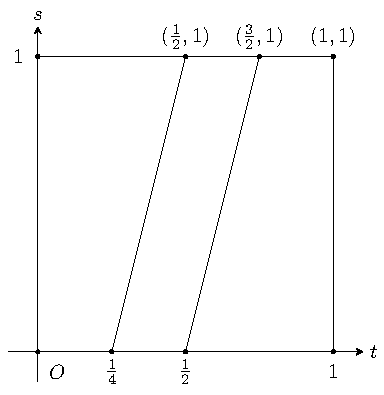
\includegraphics[scale=1]{images/fig_1.pdf}
            \end{center}
            \caption{Dominio de la función $F$.}
        \end{figure}

        para todo $s,t\in I$. Veamos que $F$ es continua... %TODO
    \end{proof}

    Para cualquier punto $x\in X$, denotemos por $\mathscr{I}_x=[i_x]$ a la clase de equivalencia del mapeo identidad, es decir $\cf{i_x}{I}{X}$ es tal que $i_x(t)=x$ para todo $y\in I$. Esta clase tiene la siguiente propiedad fundamental:

    \begin{lema}
        Sea $\mathscr{F}=[f]$ una clase de equivalencia de caminos con punto inicial $x\in X$ y terminal $y\in X$. Entonces, $\mathscr{I}_x\cdot\mathscr{F}=\mathscr{F}$ y $\mathscr{F}\cdot\mathscr{I}_y=\mathscr{F}$.
    \end{lema}

    \begin{proof}
        Solo se probará la primera igualdad, para ello, basta con probar que $i_x\cdot f\sim f$. En efecto, defina la función $\cf{F}{I\times I}{X}$ dada por:
        \begin{equation*}
            F(t,s)=\left\{
                \begin{array}{lcr}
                    x & \textup{ si } & 0\leq t\leq\frac{s}{2}\\
                    f\left(\frac{2t-s}{2-s}\right) & \textup{ si } & \frac{s}{2}\leq t\leq 1\\
                \end{array}
            \right.
        \end{equation*}
        para todo $s,t\in I$. Entonces, $F(t,0)=f(t)$ y $F(t,1)=(e\cdot f)(1)$ siendo $F$ continua. Por tanto, $\mathscr{I}_x\cdot\mathscr{F}=\mathscr{F}$.
    \end{proof}

    En cierto modo, lo que decimos es que la clase $\mathscr{I}_x$ actúa como elemento identidad (\textit{¿De dónde?}).

    \begin{mydef}
        Para cualquier camino $\cf{f}{I}{X}$, $\overline{f}$ denota al camino definido por:
        \begin{equation*}
            \overline{f}(t)=f(1-t),\quad\forall t\in I
        \end{equation*}
        El camino $\overline{f}$ se obtiene recorriendo el camino $f$ en sentido contrario.
    \end{mydef}

    \begin{lema}
        Sea $f$ un camino y denotemos por $\mathscr{F}=[f]$ y $\overline{\mathscr{F}}=[\overline{f}]$, entonces:
        \begin{equation*}
            \mathscr{F}\cdot\overline{\mathscr{F}}=\mathscr{I}_x\quad\textup{y}\quad\overline{\mathscr{F}}\cdot\mathscr{F}=\mathscr{I}_y
        \end{equation*}
        donde $x\in X$ y $y\in X$ son los puntos inicial y terminal de $f$, respectivamnete.
    \end{lema}

    \begin{proof}
        Sólo se probará la primera igualdad, para ello es suficiente con probar que $f\cdot\overline{f}\sim i_x$. Definimos la función $\cf{F}{I\times I}{X}$ por:
        \begin{equation*}
            F(t,s)=\left\{
                \begin{array}{lcr}
                    f(2t) & \textup{ si } & 0\leq t\leq\frac{s}{2}\\
                    f(s) & \textup{ si } & \frac{s}{2}\leq t\leq1-\frac{s}{2}\\
                    f(2-2t) & \textup{ si } & 1-\frac{s}{2}\leq t\leq1\\
                \end{array}
            \right.
        \end{equation*}
        para todo $s,t\in I$. Entonces,
        \begin{equation*}
            \begin{split}
                F(t,0)&=\left\{
                    \begin{array}{lcr}
                        f(2t) & \textup{ si } & 0\leq t\leq0\\
                        f(s) & \textup{ si } & 0\leq t\leq1-0\\
                        f(2-2t) & \textup{ si } & 1-0\leq t\leq1\\
                    \end{array}
                \right.\\
                &=\left\{
                    \begin{array}{lcr}
                        f(0) & \textup{ si } & t=0\\
                        f(0) & \textup{ si } & 0\leq t\leq1\\
                        f(2-2t) & \textup{ si } & t=1\\
                    \end{array}
                \right.\\
                &=\left\{
                    \begin{array}{lcr}
                        x & \textup{ si } & 0\leq t\leq1\\
                        f(0) & \textup{ si } & t=1\\
                    \end{array}
                \right.\\
                &=x\\
            \end{split}
        \end{equation*}
        para todo $t\in I$. Además,
        \begin{equation*}
            \begin{split}
                F(t,1)&=\left\{
                    \begin{array}{lcr}
                        f(2t) & \textup{ si } & 0\leq t\leq\frac{1}{2}\\
                        f(1) & \textup{ si } & \frac{1}{2}\leq t\leq1-\frac{1}{2}\\
                        f(2-2t) & \textup{ si } & 1-\frac{1}{2}\leq t\leq1\\
                    \end{array}
                \right.\\
                &=\left\{
                    \begin{array}{lcr}
                        f(2t) & \textup{ si } & 0\leq t\leq\frac{1}{2}\\
                        f(1-(2t-1)) & \textup{ si } & \frac{1}{2}\leq t\leq1\\
                    \end{array}
                \right.\\
                &=\left\{
                    \begin{array}{lcr}
                        f(2t) & \textup{ si } & 0\leq t\leq\frac{1}{2}\\
                        \overline{f}(2t-1) & \textup{ si } & \frac{1}{2}\leq t\leq1\\
                    \end{array}
                \right.\\
                &=f\cdot\overline{f}(t)\\
            \end{split}
        \end{equation*}
        para todo $t\in I$. La función $F$ es continua... %TODO

        Por tanto, $\mathscr{F}\cdot\overline{\mathscr{F}}$.
    \end{proof}

    En visata de estas propiedades de la clase $\overline{\mathscr{F}}$, de ahora en adelante la denotaremos por $\mathscr{F}^{-1}$.

    Podemos resumir todos los lemas antes probados diciendo que el conjunto de todas las clases de caminos en un espacio $X$ satisfacen los axiomas de grupo, excepto que el producto de dos caminos no siempre está definido. Solventamos este problema con la siguiente definición:

    \begin{mydef}
        Un camino o una clase de camino es llamada \textbf{cerrada} o un \textbf{bucle}, si el punto inicial y terminal son el mimso. El bucle se dice que tiene \textbf{base} en el punto inicial o terminal.
    \end{mydef}

    \begin{theor}
        Sea $X$ un espacio topológico y $x\in X$ un punto fijo. Entonces, el conjunto de todas las clases de caminos cerradas que tienen como punto base a $x$ dotado por la operación $\cdot$, denotado por $\pi(X,x)$ es un grupo llamado \textbf{grupo fundamental} o \textbf{grupo de Poincaré} de $X$ con punto base $x$.
    \end{theor}

    \begin{proof}
        Es un resumen de todos los lemas anteriores.
    \end{proof}

    \begin{obs}
        Para un espacio topológico dado $X$ y $x\in X$, dotamos el grupo fundamental $\pi(X,x)$ de una operación binaria que lo hace de grupo, de ahora en adelante tal operación se denotará al producto de dos clases $[f]$ y $[g]$ por $[f]\cdot[g]$ o por yuxtaposición como $[f][g]=[f\cdot g]$ (no confundir la operación dentro de los paréntesis cuadrados con la composición usual de funciones).

        Si $[f]\in\pi(X,x)$, se denotará a su inverso por $[f]^{-1}$ y, al elemento identidad por $\mathscr{I}$
    \end{obs}

    \begin{propo}
        Sea $X$ un espacio y $x,y\in X$ dos puntos distintos. Si $\cf{\gamma}{I}{X}$ es un camino con punto inicial $x$ y terminal $y$, entonces $\pi(X,x)\cong\pi(X,y)$ (es decir, son grupos isomorfos).
    \end{propo}

    \begin{proof}
        En efecto, defina la función $\cf{u}{\pi(X,x)}{\pi(X,y)}$ dada por:
        \begin{equation*}
            u([f])=[\gamma]^{-1}[f][\gamma]
        \end{equation*}
        Por cursos anteriores de teoría de Grupos, se ve de forma inmediata que esta función es un isomorfismo entre los grupos $\pi(X,x)$ y $\pi(X,y)$.
    \end{proof}

    \begin{cor}
        Sea $X$ un espacio topológico arco-conexo, entonces los grupos $\pi(X,x)$ y $\pi(X,y)$ son isomorfos para todo $x,y\in X$.
    \end{cor}

    La importancia del teorema anterior radica en que el grupo $\pi(X,x)$ tiene propiedades como grupo (es decir, es abeliano, finito, nilpotente, libre, etc...) no debido al punto elegido $x\in X$, sino al espacio mismo $X$, suponiendo que $X$ es arco-conexo.

    En general, no hay un mapeo canónico o isomorfismo natural entre $\pi(X,x)$ y $\pi(X,y)$, ya que a cada elección de camino entre $x$ y $y$ le corresponderá un isomorfismo.

    \section{Efecto de una función continua en el grupo fundamental}

    \begin{obs}
        Para esta sección resultará de utilidad definir el siguiente conjunto, para todo espacio topológico $X$ se define
        \begin{equation*}
            \wp_X = \bigcup \left\{[f]\Big|\cf{f}{I}{X}\textup{ es una función continua} \right\}
        \end{equation*}
        es decir, estamos tomando todas las clases de caminos de un espacio topológico $X$ (note que no tiene nada que ver con el grupo fundamental, más que con el hecho de que usa las clases de caminos en su definición).
    \end{obs}

    Considere dos espacios topológicos $X$ y $Y$ y sea $\cf{\varphi}{X}{Y}$ una función continua. Si $\cf{f_0,f_1}{I}{X}$ son caminos en $X$, ¿también lo son $\varphi\circ f_0$ y $\varphi\circ f_1$?

    \begin{propo}
        Sean $X$ y $Y$ espacios topológicos, $\cf{f_0,f_1}{I}{X}$ caminos equivalentes. Entonces, $\varphi\circ f_0\sim \varphi\circ f_1$.
    \end{propo}

    \begin{proof}
        Como $f_1\sim f_0$, existe pues una función continua $\cf{F}{I\times I}{X}$ tal que
        \begin{equation*}
            F(x,0)=f_0(x),\quad F(x,1)=f_1(x)
        \end{equation*}
        para todo $x\in I$ y,
        \begin{equation*}
            F(0,t)=f_0(0)=f_1(0),\quad F(1,t)=f_0(1)=f_1(1)
        \end{equation*}
        Considere la función $\cf{G}{I\times I}{Y}$ dada por:
        \begin{equation*}
            G(x,t)=\varphi\circ F(x,t)
        \end{equation*}
        Es claro que esta funciónes continua por ser composición de funciones continuas, además se cumple que
        \begin{equation*}
            \begin{split}
                G(x,0)&=\varphi\circ F(x,0)\\
                &=\varphi (F(x,0))\\
                &=\varphi (f_0(x))\\
                &=\varphi\circ f_0(x)\\
            \end{split}
        \end{equation*}
        para todo $x\in I$. De forma análoga
        \begin{equation*}
            G(x,1)=\varphi\circ f_1(x)
        \end{equation*}
        La otra condición se verifica de forma inmediata, con lo que se concluye que $\varphi\circ f_0\sim \varphi\circ f_1$.
    \end{proof}

    Con la proposición anterior, podemos definir sin problemas una función que mapee clases de caminos en $X$ a clases de caminos en $Y$, a partir de la función continua $\varphi$. Esto se hará con el objetivo de ver qué sucede con el grupo fundamental bajo esta función continua $\varphi_*$.

    \begin{mydef}
        Sean $X$ y $Y$ espacios topológicos y $\cf{\varphi}{X}{Y}$ una función continua. Sea $\cf{f}{I}{X}$ un camino que une a los puntos $x,y\in X$, se define la función $\cf{\varphi_*}{\wp_X}{\wp_Y}$ por
        \begin{equation*}
            \varphi_*([f])=[\varphi\circ f]
        \end{equation*}
        por la proposición anterior, esta función está bien definida.
    \end{mydef}

    Ahora, analizaremos las propiedades de la función $\varphi_*$.
    
    \renewcommand{\theenumi}{\roman{enumi}}

    \begin{propo}
        Sean $X$ y $Y$ espacios topológicos y $\cf{\varphi}{X}{Y}$ una función continua.
        \begin{enumerate}
            \item Si $\cf{f_0,f_1}{I}{X}$ son caminos en $X$ tales que $f_0\cdot f_1$ está definido (por ende, $[f_0]\cdot [f_1]$ lo está), entonces $\varphi_*([f_0]\cdot[f_1])=\varphi_*([f_0])\cdot\varphi_*([f_1])$.
            \item Para cualquier punto $x\in X$, $\varphi_*(\mathscr{I}_x)=\mathscr{I}_{\varphi(x)}$.
            \item Si $\cf{f}{I}{X}$ es un camino, entonces $\varphi_*([f]^{-1})=(\varphi_*([f]))^{-1}$.
        \end{enumerate}
    \end{propo}

    \begin{proof}
        De (i): Veamos primero que el producto $\varphi_*([f_0])\cdot\varphi_*([f_1])$ está bien definido. En efecto, dado a que el producto $[f_0]\cdot [f_1]$ lo está, entonces
        \begin{equation*}
            f_0(1)=f_1(0)
        \end{equation*}
        luego,
        \begin{equation*}
            \varphi\circ f_0(1)=\varphi\circ f_1(0)
        \end{equation*}
        donde $\varphi_*([f_0])=[\varphi\circ f_0]$ y $\varphi_*([f_1])=[\varphi\circ f_1]$, por tanto el producto de ambas clases está definido. Probemos ahora la igualdad. Se tiene que
        \begin{equation*}
            \begin{split}
                \varphi_*([f_0]\cdot[f_1])&=\varphi_*([f_0\cdot f_1])\\
                &=[\varphi\circ (f_0\cdot f_1)]\\
            \end{split}
        \end{equation*}
        siendo
        \begin{equation*}
            f_0\cdot f_1(t)=\left\{
                \begin{array}{lcr}
                    f_0(2t) & \textup{ si } 0\leq t\leq \frac{1}{2}\\
                    f_1(2t-1) & \textup{ si } \frac{1}{2}\leq t\leq 1\\
                \end{array}
            \right.,\quad\forall t\in I
        \end{equation*}
        por ende,
        \begin{equation*}
            \begin{split}
                \varphi\circ (f_0\cdot f_1)(t)&=\left\{
                    \begin{array}{lcr}
                        \varphi(f_0(2t)) & \textup{ si } 0\leq t\leq \frac{1}{2}\\
                        \varphi(f_1(2t-1)) & \textup{ si } \frac{1}{2}\leq t\leq 1\\
                    \end{array}
                \right.\\
                &=\left\{
                    \begin{array}{lcr}
                        \varphi\circ f_0(2t) & \textup{ si } 0\leq t\leq \frac{1}{2}\\
                        \varphi\circ f_1(2t-1) & \textup{ si } \frac{1}{2}\leq t\leq 1\\
                    \end{array}
                \right.\\
                &=(\varphi\circ f_0)\cdot (\varphi\circ f_1)(t),\quad\forall t\in I\\
            \end{split}
        \end{equation*}
        luego entonces
        \begin{equation*}
            \begin{split}
                [\varphi\circ (f_0\cdot f_1)]&=[(\varphi\circ f_0)\cdot (\varphi\circ f_1)]\\
                &=[\varphi\circ f_0]\cdot [\varphi\circ f_1]\\
                &=\varphi_*([f_0])\cdot \varphi_*([f_1])\\
            \end{split}
        \end{equation*}
        lo que prueba el resultado.

        De (ii) y (iii): Ejercicio.
    \end{proof}

    Por estas razones, llamaremos a $\varphi_*$ un \textit{homomorfismo} u \textit{homomorfismo inducido por $\varphi$}.

    \begin{propo}
        En el contexto de la proposición anterior, si $Z$ es un espacio topológico y $\cf{\psi}{Y}{Z}$ es una función continua, entonces
        \begin{equation*}
            (\psi\circ\varphi)_*=\psi_*\circ\varphi_*
        \end{equation*}
    \end{propo}

    \begin{proof}
        Es claro que la composición de ambas funciones está bien definida. Probaremos ahora la igualdad, sea $\cf{f}{I}{X}$ un camino, entonces:
        \begin{equation*}
            \begin{split}
                (\psi\circ\varphi)_*([f])&=[\psi\circ\varphi\circ f]\\
                &=[\psi\circ(\varphi\circ f)]\\
                &=\psi_*([\varphi\circ f])\\
                &=\psi_*(\varphi_*([f]))\\
                &=\psi_*\circ \varphi_*([f])\\
            \end{split}
        \end{equation*}
        lo que prueba la igualdad.
    \end{proof}

    \begin{excer}
        Sea $X$ espacio topológico y $\cf{i}{X}{X}$ la función identidad, entonces
        \begin{equation*}
            i_*([f])=[f]
        \end{equation*}
        para todo camino $\cf{f}{I}{X}$ en $X$.
    \end{excer}

    \begin{proof}
        Ejercicio.
    \end{proof}

    \begin{cor}
        Sean $X$ y $Y$ espacios topológicos y $\cf{\varphi}{X}{Y}$ una función continua y $x\in X$. La función $\varphi_*$ restringida a $\pi(X,x)\subseteq\wp_X$ es un homomorfismo entre $\pi(X,x)$ y $\pi(Y,\varphi(x))$. Más aún, si $\varphi$ es homeomorfismo, entonces $\varphi_*$ es isomorfismo.
    \end{cor}

    \begin{proof}
        
    \end{proof}

    \section{Nociones geométricas subyacentes}

    Para continuar con el estudio de la función inducida $\varphi_*$, es necesario introducir algunos conceptos geométricos relevantes,

    \begin{mydef}
        Sean $X$ y $Y$ espacios topológicos. Dos funciones continuas $\cf{\varphi_0,\varphi_1}{X}{Y}$ son \textbf{homotópicas} si existe una función continua $\cf{\Phi}{X\times I}{Y}$ tal que para todo $x\in X$:
        \begin{equation*}
            \Phi(x,0)=\varphi_0(x)\quad\textup{y}\quad\Phi(x,1)=\varphi_1(x)
        \end{equation*}
        además, para denotar que son homotópicas, se usará el símbolo $\varphi_0\simeq\varphi_1$.
    \end{mydef}

    \begin{propo}
        Sean $X$ y $Y$ espacios topológicos. Considere el conjunto:
        \begin{equation*}
            \mathcal{F}=\left\{\cf{\varphi}{X}{Y}\Big|f\textup{ es una función continua} \right\}
        \end{equation*}
        entonces, $\simeq$ es una relación de equivalencia sobre $\mathcal{F}$.
    \end{propo}

    \begin{proof}
        Ejercicio.
    \end{proof}

    \begin{obs}
        Para aquellos que han tomado algún curso en teoría de categorías, verán de forma casi inmediata que esta relación de equivalencia induce una partición en la clase de todos los morfismos entre espacios topológicos.
    \end{obs}

    La idea detrás de la homotopía es intentar deformar de forma continua una función en la otra, conservando la continuidad de las funciones, veamos que si
    \begin{equation*}
        \varphi_t(x)=\Phi(x,t)
    \end{equation*}
    para todo $x\in X$ y todo $t\in I$, entonces la función $\cf{\varphi_t}{X}{Y}$ es continua.

    Por esta razón es que comúnmente se habla de homotopía como la deformación continua de una función.

    \begin{obs}
        En otros contextos, resulta más familiar decir que dos funciones son homotópicas si pueden ser unidas con un arco en el espacio de todas las funciones continuas que van de $X$ en $Y$.
    \end{obs}

    \begin{mydef}
        
    \end{mydef}

    \newpage

    \section{Ejercicios}

    \begin{excer}
        Pruebe que un espacio conexo y localmente arco-conexo es arco conexo.
    \end{excer}

    \begin{proof}
        
    \end{proof}

    \begin{excer}
        ¿Bajo qué condiciones dos clases de caminos que unen a $x$ y $y$ se tendrá el mismo isomorfismo entre de $\pi(X,x)$ y $\pi(X,y)$?
    \end{excer}

    \begin{sol}
        
    \end{sol}

    \begin{excer}
        Sea $X$ un espacio arco conexo. ¿Bajo qué condiciones es la siguiente proposición válida? Para cualesquiera dos puntos $x,y\in X$ todas las clases de caminos de $x$ a $y$ dan el mismo isomorfismo entre $\pi(X,x)$ y $\pi(X,y)$. 
    \end{excer}

    \begin{sol}
        
    \end{sol}

    \begin{excer}
        Sean $\cf{f,g}{I}{X}$ dos caminos con punto inicial $x_0$ y final $x_1$. Pruebe que $f\sim g$ si y sólo si $f\cdot\overline{g}$ es equivalente al camino constante en $x_0$ (recordando que $\overline{g}$ es el camino que invierte la forma de recorrer a $g$).
    \end{excer}

    \begin{proof}
        
    \end{proof}

    \begin{excer}
        Sean $\cf{\varphi}{X}{Y}$ una función continua y $[f]$ una clase de camino en $X$ que va de $x_0$ a $x_1$. Pruebe que el siguiente diagrama es conmutativo:
        \begin{equation*}
            \begin{array}{rcccl}
              & \pi(X,x_0) & \overset{\varphi_*}{\longrightarrow} & \pi(Y,\varphi(x_0)) & \\
              u & \downarrow & & \downarrow & v \\
               & \pi(X,x_1) & \overset{\varphi_*}{\longrightarrow} & \pi(Y,\varphi(x_1)) & \\
            \end{array}
        \end{equation*}
        donde $u$ es el homomorfismo definido como: $u([g])=[f]^{-1}\cdot[g]\cdot[f]$ y $v$ se define de forma similar usando $\varphi_*([f])$ en lugar de $[f]$. ¿Qué sucede si $\varphi(x_0)=\varphi(x_1)$?
    \end{excer}

    \begin{proof}
        
    \end{proof}

    \begin{excer}
        Construya una deformación de retracción de $\mathbb{R}^n$ en $S^{ n-1}$.
    \end{excer}

    \begin{sol}
        
    \end{sol}
    
\end{document}